\chapter{Executive Summary}
\label{ch:exec-summ}

The aim of this volume of the DUNE Technical Design Report
(TDR) is to describe in detail the science program of DUNE.
In addition to description of identified scientific opportunities
and key goals, accomplishing this aim necessarily entails
presentation of the best current understanding
of the capability of DUNE to realize these opportunities,
along with the justifications on which it is based.

Within the context of the complete set of DUNE TDR volumes,
a central role for this volume is to document the scientific
basis underlying the conception and design of the LBNF/DUNE
experimental configurations.  As a result, it is the
description of DUNE's experimental capabilities that comprises
the bulk of the document.  Key linkages between requirements for
successful execution of the physics program and
primary specifications of the experimental configurations
are drawn and summarized.

This document serves a wider purpose as a statement on the
scientific potential of DUNE as a central component within
a global program of frontier theoretical and experimental
particle physics research. Thus, the presentation also
aims to serve as a resource for
the particle physics community at large.

In this chapter,
the scientific goals, the methodologies utilized to obtain
sensitivity projections, the corresponding results
for selected elements of the scientific program, and
the demands placed on the experiment design and performance
are presented in summary form.  The DUNE program is also
placed within the global scientific landscape.
Together with the two chapters that follow,
this summary establishes the context for the
detailed presentations specific to each area of
research that comprise the remaining chapters.

%%%%%%%%%%%%%%%%%%%%%%%%%%%%%%%%%%%%%%%%%%%%%%%%%%%%%%%%%%%%%%                      

\section{Overview of DUNE and its Science Program}
\label{sec:exec-program-overview}

The Deep Underground Neutrino Experiment (DUNE) will be a
world-class neutrino observatory and nucleon decay detector
designed to answer
fundamental questions about the nature of elementary particles
and their role in the universe. The international DUNE
experiment, hosted by the U.S. Department of Energy's \fnal{},
will consist of a far detector to be located about \SI{1.5}{km}
underground at the Sanford Underground Research Facility
(\surf) in South Dakota, USA, at a distance of  \SI{1300}{\km}
from \fnal{}, and a near detector to be located at \fnal in
Illinois. The far detector will be a very large, modular
liquid argon time-projection chamber (\lartpc) with a
\fdfiducialmass fiducial mass. This \lar technology will make
it possible to reconstruct neutrino interactions
with image-like precision.

The far detector will be exposed to the world's most intense 
neutrino beam originating at \fnal{}. A high-precision near 
detector, located \SI{575}{m} from the neutrino source on 
the \fnal site, will be used to characterize
the intensity and energy spectrum of this wide-band 
beam in real time.  Over the long term, the near detector 
will also enable many strategies for mitigating systematic 
errors, both through cancellation of errors common to both near and far detectors, as well as through dedicated studies
of neutrino interactions, beam line characteristics, 
absolute reconstructed energy scale errors, to name a few.

In this section, the goals of the DUNE science program are
enumerated.  Assumptions and methods utilized in determining
DUNE's capabilities to meet these goals are summarized,
with more detail appearing in Chapter~\ref{ch:tools}.
Finally, experimental sensitivities for selected
physics measurements are shown to illustrate the level of 
performance the DUNE science collaboration has been able 
to demonstrate thus far.

%%%%%%%%%%%%%%%%%%%%%%%%%%%%%%%%%%%%%%%%%%%%%%%%%%%%%%%%%%%%%%                                   
\subsection{Key goals of DUNE science program}
\label{sec:exec-key-goals}

The LBNF/DUNE strategy has been developed to meet the
requirements set by Particle Physics Project Prioritization Panel
(P5) in 2014. It also takes into account the recommendations
of the European Strategy for Particle Physics (ESPP) adopted
by the CERN Council in 2013, which classified the \dword{lbl}
neutrino program as one of the four scientific objectives that
require international infrastructure.

As a benchmark, the P5 report~\cite{p5report} set the goal of
reaching a sensitivity to \dword{cpv} of better than three
standard deviations (\num{3}$\sigma$) over more than $75\%$
of the range of possible values of the unknown
\dshort{cp}-violating phase \deltacp.
Based partly on this goal, it stated that ``the
minimum requirements to proceed are the identified capability
to reach an exposure of \num{120}~\ktMWyr{} by the 2035 time
frame, the far detector situated underground with cavern space
for expansion to at least \fdfiducialmass \lar fiducial volume,
and \SI{1.2}{MW} beam power upgradeable to multi-megawatt power.
The experiment should have the demonstrated capability to
search for \dwords{snb} and for proton decay, providing a
significant improvement in discovery sensitivity over current
searches for the proton lifetime.''
These requirements are discussed below and in the sections
that follow.

To summarize, the DUNE experiment will combine the world's most
intense neutrino beam, a deep underground site, and massive \lar
detectors to enable a broad science program addressing some of
the most fundamental questions in particle physics.
This program is articulated in brief form below.

The primary science goals of DUNE are to:
\begin{itemize}

\item Carry out a comprehensive program of neutrino oscillation measurements using
      \numu and \anumu beams from \fnal. This program includes measurements of
      the \dword{cp} phase, determination of the neutrino mass ordering
      (the sign of \dm{31}$ \equiv m_3^2-m_1^2$), measurement of the mixing
      angle $\theta_{23}$ and the determination of the octant in which this
      angle lies, and sensitive tests of the three-neutrino paradigm.
      Paramount among these is the search for \dword{cpv} in neutrino oscillations, potentially offering 
      insight into the origin of the matter-antimatter asymmetry,
      one of the fundamental questions in particle physics and cosmology.

\item Search for proton decay in several important decay modes.
      The observation of proton decay would represent a ground-breaking discovery
      in physics, providing a key requirement for grand unification of the forces.

\item Detect and measure the $\nu_\text{e}$ flux from a core-collapse
      supernova within our galaxy, should one occur during the lifetime
      of the DUNE experiment. Such a measurement would provide a wealth
      of unique information about the early stages of core-collapse, and
      could even signal the birth of a black hole.

\end{itemize}

The intense neutrino beam from LBNF, the massive DUNE \lartpc
far detector, and the high-resolution DUNE near detector will also
provide a rich ancillary science program, beyond the primary goals
of the experiment. The ancillary science program includes:
\begin{itemize}

\item Other accelerator-based neutrino flavor transition measurements with
      sensitivity to beyond the standard model (BSM) physics, such as non-standard
      interactions (NSIs), Lorentz invariance violation, \dword{cpt} violation,
      sterile neutrinos, large extra dimensions, heavy neutral leptons,
      and measurements of tau neutrino appearance;

     \item Measurements of neutrino oscillation phenomena using atmospheric neutrinos;

     \item A rich neutrino interaction physics program utilizing the DUNE near detector,
           including a wide-range of measurements of neutrino cross sections, studies of
           nuclear effects; and

     \item Searches for dark matter utilizing a variety of
           signatures in both
           near and far detectors, as well as  
           non-accelerator searches for BSM physics 
           such as neutron-antineutron oscillation.

\end{itemize}

Further advancements in the \lartpc %far detector 
technology during the course of the far detector construction
may enhance DUNE's capability to observe very low-energy
phenomena such as solar neutrinos or even the diffuse
supernova neutrino flux.

%%%%%%%%%%%%%%%%%%%%%%%%%%%%%%%%%%%%%%%%%%%%%%%%%%%%%%%%%%%%%%                                   
\subsection{Summary of assumptions and methods employed}
\label{sec:exec-assm-meth}

Scientific capabilities are determined assuming DUNE
is configured according to the general parameters described above.
%(Sec.~\ref{sec:exec-program-overview}),
Further assumptions regarding the neutrino beam and detector 
systems, and their deployment, are stated here in
Sections~\ref{sec:exec-assm-meth-beamdetector} and
\ref{sec:exec-assm-meth-deployment}.  More detail is given
in later chapters as appropriate.

Determination of experimental sensitivities relies on the
modeling of the underlying physics and background processes,
as well as the detector response, including calibration and
event reconstruction performance and the utilization of data
analysis techniques and tools.
While a brief discussion of the strategies employed is given below
in Sec.~\ref{sec:exec-assm-meth-simreco}, a dedicated chapter
(\ref{ch:tools}) is devoted to the presentation of this material.
Considerations specific to individual elements of the science
program are presented in detail in the corresponding chapters.

\subsubsection{Beam and Detector}
\label{sec:exec-assm-meth-beamdetector}

This document presents physics sensitivities using
the optimized design of the 1.2~MW neutrino beam and
corresponding protons-on-target per year assumed to
be 1.1 $\times 10^{21}$ POT.  These numbers assume a combined
uptime and efficiency of the \fnal accelerator complex and the
LBNF beamline of 56\%.  The beam design, simulation and associated
uncertainties are described in
Sec.~\ref{sec:physics-lbnosc-flux}.

For the neutrino oscillation physics program, it is assumed that
equal exposures are obtained with both horn current polarities,
and therefore with the corresponding mix of primarily \numu
and \anumu data samples (see Sec.~\ref{sec-physics-lbnosc-osc}).

It is assumed that the DUNE far detector will include some
combination of the different 10-kt fiducial volume
implementations (single and dual-phase) of the \lartpc concept
for which technical designs have been developed.
%(see Sec.~\ref{sec:exec-scope}).                                                                
For much of the science program it is expected that the
capabilities of the two proposed far detector module 
implementations will be comparable.  As a result of the
current state of reconstruction and analysis software development
(see Sec.~\ref{sec:exec-assm-meth-simreco}), the
physics sensitivity studies reported in this TDR are based on
the single-phase \lartpc implementation,
documented in full in Volume~\volnumbersp.

It is also assumed that validation of the DUNE far detector 
designs will come from data and operational experience acquired 
with the large-scale ProtoDUNE detectors staged at CERN, 
including single-particle studies of data obtained 
in test-beam running.  Although this program is in early stages, 
initial data has been collected with the ProtoDUNE-SP detector.  
Where possible preliminary results from initial analyses 
will be presented in this document (see Chapter~\ref{ch:tools}.

The near detector for DUNE has been under active development,
and a Conceptual Design Report is in preparation.
Correspondingly, the descriptions utilized in this TDR
are consistent with this level of development.  As the
beam-based neutrino oscillation program depends strongly
on the capabilities of the near detector systems, a brief
summary of these systems and their expected performance is
given in Chapter~\ref{ch:osc}.

\subsubsection{Deployment Scenario}
\label{sec:exec-assm-meth-deployment}

Where presented as a function of calendar year,
sensitivities are calculated with the following
assumed deployment plan, which is based on a
technically limited schedule.
\begin{itemize}
    \item Year 1: Two far detector (FD) volumes for total
          fiducial mass of 20 kt, 1.2 MW beam,
          initial near detector (ND) constraints
    \item Year 2: Add one FD volume for total fiducial mass of 30 kt
    \item Year 4: Add one FD volume for total fiducial mass of 40 kt,
          improved ND constraints
    \item Year 7: Upgrade to 2.4 MW beam
\end{itemize}


\subsubsection{Simulation, Reconstruction and Data Analysis Tools}
\label{sec:exec-assm-meth-simreco}

The development of algorithms and software infrastructure needed
to carry out physics sensitivity studies has been an incremental
process.  For some aspects -- for example, beam line modeling
and GeV-scale neutrino interaction simulations --
well-developed and validated (with data) software packages have
been available throughout much of DUNE's design phase.
For others, corresponding tools did not exist and needed to be
either developed from scratch or adapted with substantial
modifications from other experimental programs.  Concurrent
with these development efforts, interim descriptions such
as parametric detector response modeling, necessarily crude
but based on reasonable extrapolation from experience and
dedicated studies, were employed to assess physics capabilities.
Even for the case of the better-developed tools -- again,
neutrino interaction modeling is a good example -- incremental
improvements have been made as data from neutrino experiments
and other sources have become available and as theoretical
understandings have advanced.

Consequently, practical considerations, including computing
and human resource availability, have led to different levels
of rigor in the evaluation of physics capabilities for
different elements of the program.  The strategy adopted for
this TDR has been to hold the primary elements of the program
to the highest standard of rigor, involving direct analysis
of fully simulated data, utilizing actual event reconstruction
codes and analysis tools that could be applied to real data
from DUNE far detector modules.  For other elements of the
program, sensitivities utilize realistic beam and
physics simulations, but employ parametric detector
response models in place of full reconstruction.

The implementation of this strategy comes with caveats
and clarifications that are discussed in the corresponding
chapters.  Some of these are mentioned here.
\begin{itemize}
\item In the case of the long-baseline oscillation physics
      program, this approach has necessarily been augmented
      with the concurrent analysis of simulated data from
      near detector systems employing parametric
      detector response modeling, as described in
      Sec.~\ref{sec:nu-osc-06}.

\item In the case of the nucleon decay searches
      (Sec.~\ref{sec:nonaccel-ndk}),
      given the provisional state of development of dedicated
      reconstruction and analysis tools, this strategy exposes
      the risk that the current analyses could be considerably
      less effective than what is eventually realized,
      resulting in underestimation of physics sensitivity.

\item The above consideration is also true for the supernova
      neutrino burst program (Sec.~\ref{sec:snb-lowe-snb}),
      which relies on reconstruction of event signatures
      from \lartpc signals generated by low-energy
      (MeV-scale) particles (electrons and de-excitation gammas).
      In this case a modified strategy is employed:
      parameterized reconstruction metrics are derived from
      analysis of fully simulated low-energy events
      in the far detector to augment extrapolations
      from other experimental platforms.

\item It should be noted that for program elements where
      analysis of fully reconstructed simulated data is not
      yet possible, the parametric response models used have
      been well characterized with dedicated studies
      and incorporation of results from other experiments.
      The demonstration of sensitivities for the long-baseline
      oscillation physics program that are comparable to those
      previously obtained based on parametric response
      provides validation for this approach.
\end{itemize}


%%%%%%%%%%%%%%%%%%%%%%%%%%%%%%%%%%%%%%%%%%%%%%%%%%%%%%%%%%%%%%                                   
\subsection{Selected results from sensitivity studies}
\label{sec:exec-sensitiv-results}

\todo{This section is still in development as results from 
physics working groups are being finalized}

%%%%%%%%%%%%%%%%%%%%%%%%%%%%%%%%%%%%%%%%%%%%%%%%%%%%%%%%%%%%%%                                   
\section{Science Program Drivers for LBNF/DUNE Design Specifications}
\label{sec:exec-key-reqs}

The scientific case summarized in the sections above
is predicated on the suitability of the experimental
configuration of LBNF/DUNE.  In this section we summarize
the ways in which the primary physics goals drive key features
of this configuration.  Further elaboration of the impacts of
physics goals on specific high-level performance needs of the
experimental systems is presented in the corresponding chapters
that follow.  Translation of performance needs into the
corresponding LBNF/DUNE design specifications is addressed within
the appropriate TDR volume.

\subsection{General LBNF/DUNE Operating Principles}

World-wide scientific and technical planning for the
ambitious next-generation deep underground long-baseline
neutrino oscillation experiment that LBNF/DUNE now represents
has been under way for more than a decade.  Much
development preceded the formation of the DUNE science
collaboration in 2015 (see, for example,
Refs.~\cite{Adams:2013qkq} and \cite{LAGUNA-LBNO-deliv}).

Extensive study and discussion within the community
have led to the principal elements of the LBNF/DUNE
configuration:
\begin{itemize}
  \item {\bf\boldmath High-intensity conventional wide-band
  $\nu_\mu$ beam}\\
	The current generation of long-baseline neutrino experiments
	have benefited from narrow-band beam characteristics 
	associated with off-axis detector deployment. The principal advantage is a low background rate in both \nue appearance 
	and \numu disappearance channels from misidentified neutral current interactions of high energy neutrinos.  
	However, this advantage comes at a cost of flux and 
	spectral information relative to an on-axis detector 
    configuration~\cite{Adams:2013qkq,Agarwalla:2014tca}.
    The DUNE concept
    builds on the notion that a highly-performant detector
    technology with excellent background rejection capability can
    optimize sensitivity and cost with an on-axis exposure to
    an intense conventional (horn-focused) beam.

  \item {\bf Far detector site selection for long baseline}\\
    The 1300-km baseline offered by locating the DUNE far detector
    at the Sanford Underground Research Facility in Lead, 
    South Dakota is well-optimized for the neutrino oscillation 
    physics goals of the program~\cite{Bass:2013vcg}.

  \item {\bf Deep underground location for far detector modules}\\
    Early studies (see, {\sl e.g.}, Ref.~\cite{homestake:depth}) 
    demonstrated that to realize the non-accelerator based elements
    of the DUNE science program, a deep underground far detector
    location is required.  These studies also indicate that the 
    4850 Level of Sanford Lab provides sufficient attenuation of 
    cosmic rays in the rock above, conclusions that have been 
    supported by more recent studies (see,
    {\sl e.g.}, Refs.~\cite{bib:docdb3384,bib:docdb1752}).

  \item {\bf \lartpc technology for far detector modules}\\
    Combining intrinsic scalability with high-performance event 
    imaging, calorimetry and particle identification capabilities, 
    the liquid argon Time Projection Chamber concept was developed 
    for a broad-based underground science program matching well 
    that of DUNE.  This design choice integrates well with the
    other elements and provides valuable complementarity to other 
    existing and planned detectors pursuing many
    of the same goals.  As an example of this complementarity,
    the sensitivity of DUNE to the \nue component of supernova 
    neutrino flux, prevalent in the neutronization phase of the 
    explosion, provides distinct information relative to that 
    provided by water or organic scintillator-based detectors in 
    which \anue interactions dominate.
\end{itemize}

The scientific basis for the above foundational experimental
design choices has been examined and validated through extensive
review, undertaken at all stages of DUNE concept development.
Recent experimental and theoretical developments have only
strengthened the scientific case for DUNE and its
basic configuration.  The technical underpinnings for
these choices have also been strengthened over time through a world-wide
program of R\&D and engineering development, as described in a suite
of LBNF/DUNE project documents including this Technical Design Report, as
well as in sources describing independent experiments and development
activities.

%\subsection{Performance Requirements of LBNF/DUNE Systems}     
%
%Much of the basic design of LBNF/DUNE was driven by
%general arguments and initial studies carried out employing
%parametric detector response, utilizing performance metrics 
%based on experience from previous experiments and R\&D efforts.

\subsection{Beam Line performance requirements}

\todo{This is a placeholder.  Text under development}


\subsection{Far detector performance requirements}

The number of detector design parameters that have direct
or indirect impact on performance is large.  These design
parameters have been studied over the years by past LArTPC
experiments, by DUNE during early detector optimization work,
through the successful construction and now operation of
ProtoDUNE-SP, and through continuing studies within the
DUNE consortia and physics groups.

\subsubsection{High-level observables in the Far Detector}

DUNE's suite of physics measurements relies on a relatively small
number of event observables, through which the physics of interest
can be accessed.  Foremost are:
%                                                                                                
\begin{itemize}
\item {\bf Particle energies}  \\
Examples include the total visible energy in a supernova
neutrino interaction; the reconstructed energy of a beam
neutrino for oscillation measurements; the reconstructed
energy of a muon track in a nucleon decay candidate event.

\item {\bf Particle identification}  \\
This comes from spatial patterns and energy depositions.
Examples include photon/electron separation in the \nue{}
appearance analysis; proton/kaon separation in certain
nucleon decay channels.

\item {\bf Event time} \\
This allows for fiducialization
in the TPC, drift corrections, and macroscopic timing for
beam neutrinos and supernova neutrino bursts.
\end{itemize}



\subsubsection{Physics case studies}

\paragraph{\bf CP violation search}
The primary demonstration that the detector design meets
the physics needs is the full simulation and analysis
being documented in this TDR volume.  As shown in 
Sec.~\ref{sec:exec-sensitiv-results}, Figure~\ref{fig:deltacp}
shows a snapshot of the sensitivity obtained in this way.
Selection efficiencies and energy resolutions obtained with
the simulation exceed benchmarks obtained from previous 
studies based on parameterized detector response models.
%
\begin{comment}
Anne commented per ETW and Jon 1/25
\begin{dunefigure}
[Sensitivity for excluding
CP-conserving values of $\delta_{\rm{CP}}$ as a function
of true $\delta_{\rm{CP}}$]
{fig:deltacp}
{PRELIMINARY/Placeholder.  Sensitivity for excluding
CP-conserving values of $\delta_{\rm{CP}}$ as a function
of true $\delta_{\rm{CP}}$.  The black curve represents
the goal sensitivity as stated in the CDR.  The colored
curves represent successive improvements to the event
selection and energy reconstruction algorithms, which 
still continue.  The version labeled May~2018 
surpasses the selection efficiency and energy  
resolution goals, and this is reflected in the 
CPv reach.  Systematic uncertainty assumptions
for this plot come from the CDR.}
  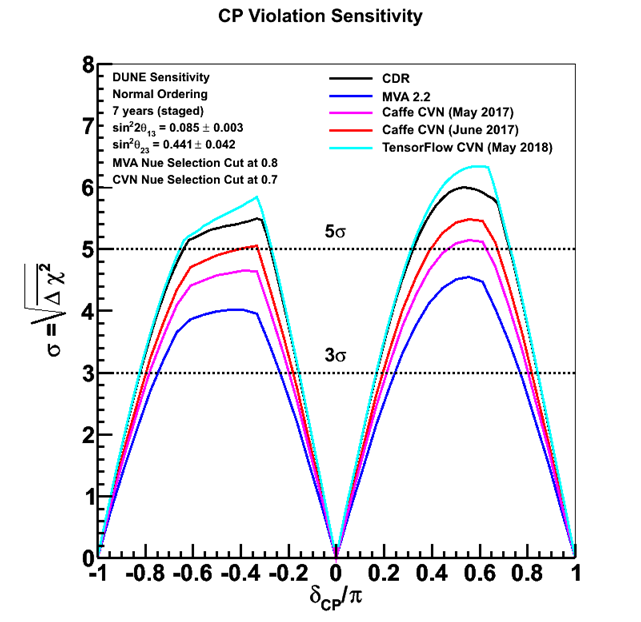
\includegraphics[width=0.7\linewidth]{deltacp.png}
\end{dunefigure}
\end{comment}
To break the measurement apart into the three
observables above, we start with neutrino energy.
The charged lepton and hadronic shower energies are
reconstructed separately and then summed.  In electron
neutrino events, the leptonic energy resolution
(spectrum averaged) is 8\%, the hadronic energy resolution
is 49\%, and the neutrino energy resolution is 13\%.
Note that a significant portion of the energy smearing
comes from the physics of neutrino-nucleus scattering
and hadronic shower production rather than from detector
performance.  In the impossible case that the lepton
energy could be perfectly reconstructed, the electron
neutrino (muon neutrino) energy resolution would only
change by approximately $13\%\rightarrow 10\%$ 
($18\%\rightarrow 17\%$).
Equivalently, small degradations in detector response
have minimal leverage to affect the final neutrino energy
resolution.

Particle identification is critical for the oscillation analysis 
in that it enables neutrino flavor identification.  
For \nue{} appearance in particular, one
must positively identify the presence of a high-energy
electron while avoiding misclassification of high energy
photons as electrons. The LArTPC design meets this challenge
by having spatial resolution that is much smaller than the
radiation length ($0.5~\rm{cm} \ll 14~\rm{cm}$) to make
visible the gaps between an event's reconstructed vertex
and any photon conversions, and charge resolution that
provides additional $dE/dx$ separation based on pre-EM-shower
depositions, as demonstrated in an operating detector by
ArgoNeuT~\cite{argoneutdedx} and with DUNE simulation
in Figure~\ref{fig:emdedx}.  The DUNE study was done as
part of the Far Detector Optimization Task Force~\cite{fdtfreport}
and thus also shows alternative detector designs for the 
single-phase \lartpc implementation.  As long as
the signal-to-noise ratio is high on the readout wires,
minor adjustments to the wire angle and pitch have negligible
impact on $dE/dx$ separation power.
%
\begin{dunefigure}
[Separation of photons and electrons by $dE/dx$
in the pre-shower region]
{fig:emdedx}
{Separation of photons and electrons by $dE/dx$
in the pre-shower region.  Alternative wire angles and wire
pitches are also shown.}
  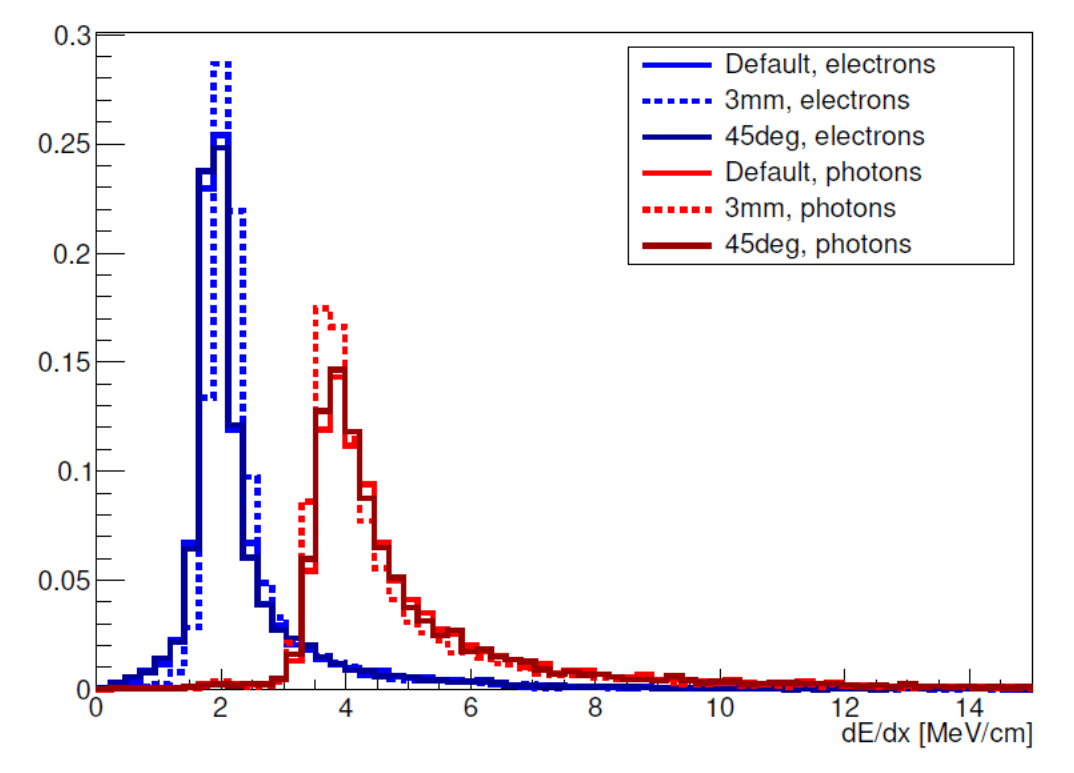
\includegraphics[width=0.7\linewidth]{emdedx.png}
\end{dunefigure}

In the analysis presented in Chapter~\ref{ch-osc}, and in
the preliminary \dword{cpv} sensitivity in
Figure~\ref{fig:deltacp}, neutrino flavor classification
is accomplished using a modern convolutional neural network
technique that takes directly as input the TPC wire hits
in the three detector views.

Event timing requirements for beam events flow from the
need to establish the fiducial volume.  This is discussed
generally in the section on light yield below.

\noindent {\bf Supernova burst neutrinos.}  A core-collapse
supernova at 10~kiloparsecs will provide $\sim$1000 neutrino
interactions in the Far Detector over the course of
$\sim$10 seconds with typical energies between 5 and 30~MeV.
Charged current \nue{} events make up the majority of these.
Much of the desired astrophysical information comes via the
time-dependent energy spectrum of these neutrinos.  As shown
earlier in Sec.~\ref{sec:exec-sensitiv-results} and later
in more detail in Chapter~\ref{ch:snb-lowe},
DUNE capabilities are quantified through sensitivities
both to generic pinched-thermal spectral parameters and to
specific phenomena within the star
({\em e.g.}, collective effects).

Figure~\ref{fig:specpars} shows the precision with which DUNE
can measure the three spectral parameters using the full
time-integrated spectrum.  The ``unit smearing'' contours
shown assume perfect neutrino energy reconstruction, with
no degradation from the neutrino interaction process itself
({\em e.g.}, energy lost to neutrons) or the detector.
The sizes of these contours are thus governed by raw event
statistics.  In an eventual detailed analysis, the spectral
fits will be done in time slices to study the evolution of
the supernova, so the minimum contour size in each time slice
will be larger due to reduced event counts in each slice.
The colored contours show increasing levels of energy smearing.
A 10\% resolution is noticeable but insignificant, and the
overall precision on the spectral parameters up to 30\%
resolution does not change dramatically, worsening in the
poorly measured high $\alpha$ region by $\sim$10\%.
A baseline energy smearing of $\mathord{\sim}5\% - 15\%$
(energy dependent) enters due to the stochastic nature of
the neutrino interaction and missing energy.  As shown later,
the additional smearing introduced by the detector's response
falls within the resolution envelope suggested here.

\begin{dunefigure}
[PRELIMINARY. 90\%~C.L.\ contours for the three
Garching pinched-thermal spectral parameters for a supernova
at 10~kpc.]
{fig:specpars}
{PRELIMINARY. 90\%~C.L.\ contours for the three
Garching pinched-thermal spectral parameters for a supernova
at 10~kpc.  The contours are obtained using the time-integrated
spectrum.  As discussed in the text, the allowed regions
change noticeably but not drastically as one moves from
no smearing (black) to various realistic resolutions (colors).
The jagged shapes in this preliminary plot are due to binning.}
  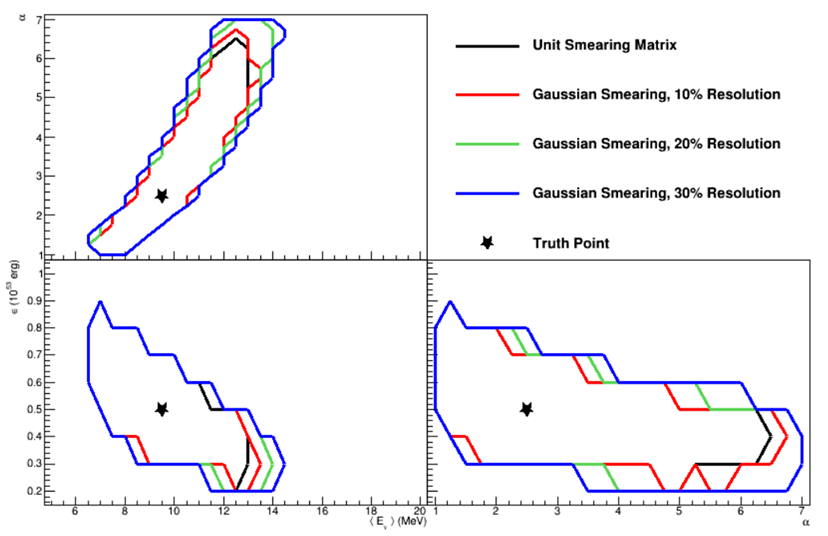
\includegraphics[width=0.7\linewidth]{specpars.png}
\end{dunefigure}

Given the dominance of \nue{} charged current events in the
supernova neutrino sample, particle identification is not a
requirement for the primary physics measurements.  However,
additional capability may be possible by identifying separately
neutral current and elastic scattering interactions.  Studies
are on-going, and these possibilities are discussed in 
Chapter~\ref{ch-snb-lowe}.

Timing for supernova neutrino events is provided by both the
TPC and the photon detector system.  Basic timing requirements
flow from event vertexing and fiducialization needs.  These are
discussed generally for DUNE in the light yield section, but
here we note a few supernova-specific design considerations.
During the first 50~ms of a 10-kpc-distant supernova, the
mean interval between successive neutrino interactions is
$0.5 - 1.7~\rm{ms}$ depending on the model.  The TPC alone
provides a time resolution of 0.6~ms (at 500~V/cm), commensurate
with the fundamental statistical limitations at this distance.
However nearly half of galactic supernova candidates lie closer
to Earth than this, so the rate can be tens or (less likely)
hundreds of times higher.  A resolution of $\mathord{<}10~\mu\rm{s}$,
as already provided by the photon detector system, ensures that
DUNE's measurement of the neutrino burst time profile is always
limited by rate and not detector resolution.  The hypothesized
oscillations of the neutrino flux due to standing accretion shock
instabilities would lead to features with a characteristic time
of $\sim$10~ms, comfortably greater than the time resolution.
The possible neutrino trapping notch at the start of the burst
has a width of $1 - 2~\rm{ms}$.  Observing the trapping notch
could be possible for the closest progenitors.

\subsubsection{Key high-level detector design specifications}

With the discussion above and in later chapters of this 
document, it is possible to identify several high-level 
detector design parameters that together characterize the  
overall function of DUNE single-phase \lartpc modules.  These 
parameters and specified operating points are given in 
Table~\ref{tab:exec-fd-specs}.
%
\begin{dunetable}[High-level DUNE single-phase far detector design specifications]
{lll}
{tab:exec-fd-specs}
{High-level DUNE single-phase far detector design parameters 
and specifications}
Parameter & Specification & Goal\\ \toprowrule
Drift field       & $>\SI{250}{\volt/\cm}$     & 500~V/cm\\
Electron lifetime & $>\SI{3}{\milli\second}$   & 10~ms\\
System noise      & $<1000$~enc & --- \\
Light yield (at cathode)  & $>\SI{0.5}{pe/\MeV}$ & $>\SI{5}{pe/\MeV}$\\
%Photon detection threshold       & $>\SI{5}{\MeV}$ &  $>\SI{0.5}{\MeV}$\\
%Light yield       & $>\SI{0.5}{pe/\MeV}$ & $>\SI{13}{pe/\MeV}$\\
Time resolution   & $<\SI{1}{\micro\second}$    & 100~ns\\
\end{dunetable}
%

The column headings in the table are defined as follows:
\paragraph{Specification:} This is the intended value for the parameter or, more often, the 
upper or lower limit for the parameter.  Fixed values are given for parameters that are not intrinsically dynamic ({\em e.g.}, wire pitch).  Limits are set by the more stringent driver, either
 the physics or engineering needs.

\paragraph{Goal:} This is an improved value that offers some benefit, and the collaboration
aims to achieve this value where it is cost effective to do so.  While in some cases the goal offers potential physics benefit directly, more often the goal provides risk mitigation, since improving the performance on one parameter can mean relaxing the requirements on other correlated parameters, thus protecting against unforeseen performance issues.

The first three parameters (drift field, electron lifetime, 
and TPC system noise) in Table~\ref{tab:exec-fd-specs} 
enter directly into the ability to discriminate between 
ionization signals due to physics events and noise.  Physics 
capability degrades if readout noise is not small compared to 
the ionization signal expected for minimum-ionizing particles
located anywhere within the active volume of the detector.
The remaining parameters (light yield for events at the cathode, 
and timing resolution) pertain to the ability 
of the scintillation photon detection system to enable 
localization of events within the TPC, needed for the 
non-accelerator based far detector physics program, both 
for fiducialization and for corrections to TPC charge 
attenuation.  The general 
arguments for the specifications listed for each parameter 
are given below.

\paragraph{Drift field}
The basic operating principle of the TPC involves the transport 
of ionization electrons out of the argon volume and to the 
detection plane.   
A higher drift field reduces electron transport time 
and thus electron loss due to impurities; 
reduces ion-electron recombination; increases induction 
signals due to increased electron velocity; and reduces 
electron diffusion.


The argon volume in the Far Detector single phase design is 
divided into four separate drift regions, each with a maximum 
drift distance of 3.5~m.  The design goal of 500~V/cm field 
implies a voltage across the drift region of approximately 
180~kV.  At this field, the electron drift velocity is 
1.6~mm/$\mu$s , implying a maximum drift time $t=2.2~\rm{ms}$.  
This drift time can be compared with the electron lifetime 
$\tau$ set by the argon purity.  At $\tau=3~\rm{ms}$, signals
originating near the cathode will be attenuated to 
$e^{-t/\tau} = 48\%$ of their original strength.  
For the minimum field of 250~V/cm, this transmission becomes 
23\%.  Additionally, electron/ion recombination happens more 
readily at lower field.  From 500~V/cm to 250~V/cm, 
an additional signal loss of 11\% (taking 23\% to 20\%) is 
introduced due to recombination.  The lowered field also 
reduces the drift velocity and, in proportion, signal pick-up 
on the induction wires.  Moving from 500~V/cm to 250~V/cm drops 
the induction signal by an additional 34\% to an effective
transmission for low-field depositions near the cathode 
(relative to ``500~V/cm near the anode'') of 14\%.

These signal attenuations are acceptable as long as the readout 
maintains good SNR and charge resolution.  High SNR for 
MIP signals has been demonstrated at ProtoDUNE-SP -- SNR=30 
(collection), 15 (induction) -- and the minimum transmissions 
above would not significantly damage the ability to identify 
wire hits.  The charge resolution on individual wires, while not 
a driver of overall event resolution, feeds into $dE/dx$ 
estimation for short segments of tracks and thus into 
particle identification.  Studies of selection efficiencies at 
varied signal levels continue, but notably the \nue 
selection efficiency exhibits no dependence on drift 
difference in the default simulation, which is based on a 
3~ms electron lifetime.  As mentioned below, ProtoDUNE readily 
achieved higher lifetimes.

Electrons drifting across the full 3.5~m will experience 
transverse diffusion of 1.7~mm (2.0~mm) at 500~V/cm (250~V/cm).  
The change in diffusion with field strength is insignificant in comparison to the wire pitch of 5~mm.

ProtoDUNE-SP is currently operating at 500~V/cm.

\paragraph{Electron lifetime}
Electronegative impurities ({\em e.g.}, $\rm{H}_{2}\rm{O}$, $\rm{O}_{2}$) within the liquid argon must be kept at 
low levels to prevent the capture of drifting electrons after ionization.  Electron lifetime is inversely proportional to the level of these impurities.

The values in Table~\ref{tab:exec-fd-specs} correspond to 
contamination levels of of 100 ppt $\rm{O}_2$-equivalent 
for 3~ms and 30~ppt for 10~ms.  The influence of electron 
lifetime on physics capabilities has been discussed in the 
section on drift field above.  
Indeed, one can largely trade off purity for field. 
Note that the lower lifetime of 3~ms was assumed throughout 
that section, versus the goal of 10~ms.  ProtoDUNE-SP has achieved electron lifetimes exceeding 5~ms.

\paragraph{Electronics system noise}
Noise in the electronics system can 
limit the ability to identify and correctly associate wire hits 
and can worsen charge resolution.  From engineering
considerations, the noise level in the front-end electronics 
drives the specification.  All other pieces of the electronics 
chain are to be kept well below this level.  
The specification is given in units of $e^-$ equivalent 
noise charge (enc).

At current gain settings, 1000~enc corresponds 
to 6.5 ADC counts.  Initial ProtoDUNE analyses are 
showing 3.5 (4.5) ADC counts on collection (induction) channels. 
The current FD simulation assumes a noise level similar to 
ProtoDUNE performance, but higher noise levels are being 
explored.  It is not expected that these relatively small
adjustments (factor of $\sim$2) will impact physics analysis 
in any significant way.  Noise assumptions (level and 
correlations) do influence DAQ design choices.

\paragraph{Light yield and photon-based timing}
The photon detector system provides an event time 
based on the scintillation light produced in the liquid argon.  
In conjunction with the TPC ionization signal, this allows 
one to determine where the event occurred along 
the drift direction for event vertexing, fiducialization, 
and electron attenuation corrections.  The 
specifications here are given for the worst-case event 
location in the fiducial volume, typically near the cathode 
and thus far from any photon detector on the anode planes.

A photon-based time resolution of 1~$\mu$s corresponds to the 
time resolution for single TPC wire hits, allowing for useful 
event matching between the TPC and photon detector systems.  
Given the drift velocity, 1~$\mu$s also corresponds to an 
effective spatial granularity in the drift direction 
($\sim$2~mm) that is similar to the wire pitch.  The resulting 
three-dimensional event vertex provided by combining TPC and 
photon detector information has essential uses in DUNE physics 
analyses.  A fiducial volume must be defined at the 
$\mathord{<}1\%$ level for the accelerator-based neutrino 
oscillation measurements and for nearby supernovas, and at less 
stringent levels for other measurements.  Additionally, most 
cosmogenic and environmental backgrounds for non-accelerator 
measurements ({\em e.g.}, neutral particles produced by cosmic 
rays in the surrounding rock) have tell-tale distributions in the
active volume and can thus be mitigated or eliminated through 
event localization.

The precise event time, and thus event location, also allows a 
correction for electron attenuation, which otherwise could have 
a large effect on energy resolutions due to the non-uniformity
of response across the drift volume.  
The minimum TPC performance 
considered (with $E=250~\rm{V/cm}$, $\tau=3~\rm{ms}$) would 
correspond to an energy smearing of 22\% due to electron loss.  
This effect is made negligible at 1~$\mu$s time resolution.

This attenuation correction is only possible when photon signals can be successfully associated with a TPC-recorded event.  For low energy supernova neutrino events, this association is not 
100\% efficient.  Figure~\ref{fig:tpcres} shows the smearing on visible energy in the TPC for supernova neutrino events with and without a drift correction based on different photon detector system performance.  The difference between no correction and any correction is dramatic.  The small differences between different light levels (cast as effective photodetector area in the figure) stem not from improved spatial resolution but from a higher efficiency at reconstructing and associating light signals with the TPC signals.  An effective area of 23~$\rm{cm}^2$ corresponds roughly to a light yield of 0.5~p.e./MeV at the cathode, {\em i.e.}\ the minimum specification.
%
\begin{dunefigure}
[Dependence of reconstructed supernova neutrino event energy on timing-based drift correction]
{fig:tpcres}
{Energy residuals for supernova neutrino events without (black) 
and with (color) a timing-based drift correction to the 
reconstructed energy.  The red histogram assumes the event 
vertex is known perfectly, and the realistic cases approach that
ideal quickly.  The $23~\rm{cm}^2$ histogram roughly corresponds 
to the specification of 0.5~p.e./MeV.}
  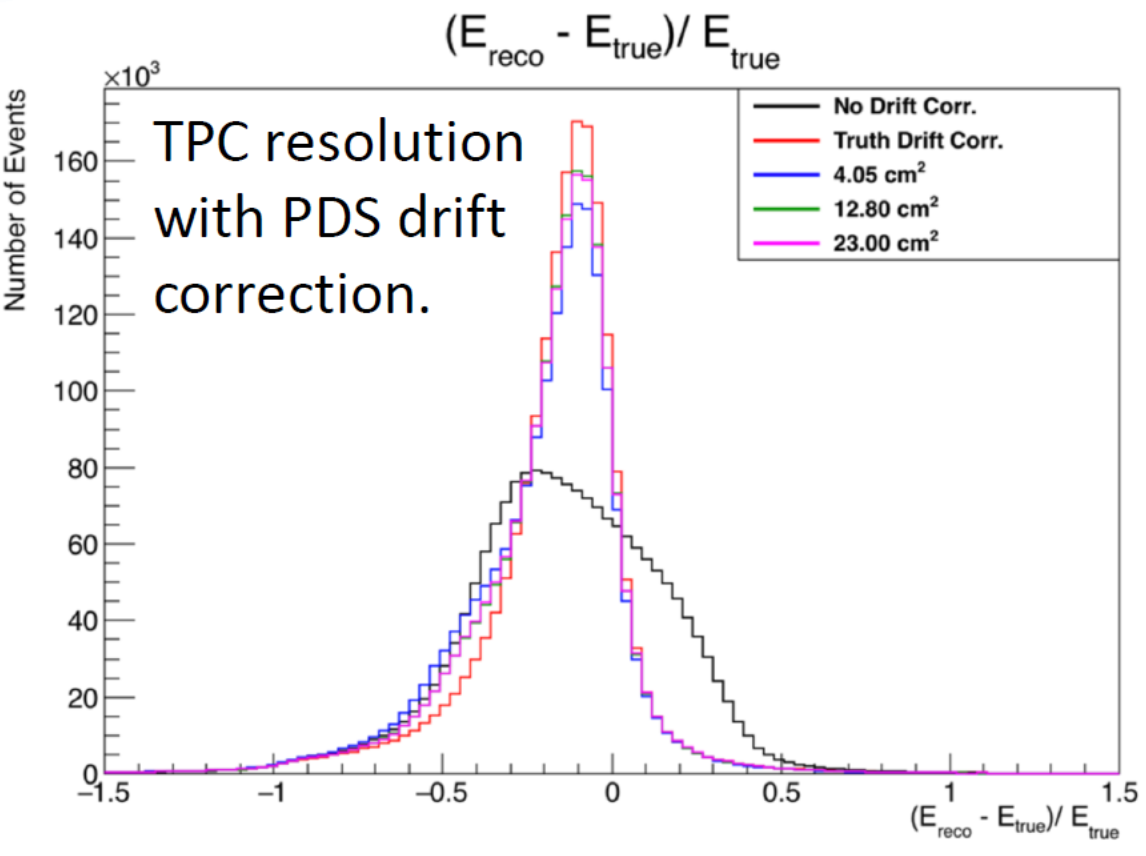
\includegraphics[width=0.7\linewidth]{tpcres.png}
\end{dunefigure}

The use of photon signals for direct event calorimetry in 
supernova neutrino events is under study. Initial tests suggest 
resolutions around 25\% are possible at 0.5 p.e./MeV, which is
competitive with the TPC resolution at these energies.

Two light-collection bar designs and one segmented design 
(ARAPUCA) are operating in ProtoDUNE-SP.  Initial performance 
evaluation is excellent, and a full quantitative assessment, 
described in Volume~\volnumbersp
is in progress.

\subsubsection{Detector Design Driver Summary}

The above discussion provides the basic guidelines for key far 
detector performance specifications in the context of the 
single-phase module design.  Further elaboration is given in the 
chapters devoted to science capabilities in this document.  
Discussion of other significant detector specifications 
and their impact on 
physics sensitivity is given in Volumes~\volnumbersp and 
\volnumberdp.  While it is not practical to carry out 
comprehensive physics sensitivity studies comprehensively, in 
which every major detector parameter is varied individually or 
in conjunction with others, such studies have been done 
for a few significant parameters (such as anode wire pitch for 
the single-phase \lartpc design).  These are reported in the 
corresponding detector volume.

%%%%%%%%%%%%%%%%%%%%%%%%%%%%%%%%%%%%%%%%%%%%%%%%%%%%%%%%%%%%%%  

\section{LBNF and DUNE in the Global Context}
\label{sec:exec-glob-context}

\todo{Placeholder section for now.  Not for inclusion in 2nd draft}

%%%%%%%%%%%%%%%%%%%%%%%%%%%%%%%%%%%%%%%%%%%%%%%%%%%%%%%%%%%%%%                                   
\section{Outlook: Impacts of DUNE Science}
\label{sec:exec-impacts}

\todo{Placeholder section for now.  Not for inclusion in 2nd draft}


%%%%%%%%%%%%%%%%%%%%%%%%%%%%%%%%%%%%%%%%%%%%%%%%%%%%%%%%%%%%%%                                   
\section{Scope and Organization of this Document}
\label{sec:exec-scope}

The scope and organization of this document follow from
both programmatic and practical considerations.

First, while this volume is strongly interconnected with
the other TDR volumes, it is written so as to stand on its
own to a reasonable extent, in order to be of best use to the
community outside DUNE.  To accomplish this, some duplication
of material presented in other volumes is unavoidable.
At the same time, the full utility of this volume
is as just one element within an integrated set of TDR volumes.
Thus, explicit and implicit reference
to material presented in other volumes is made freely.

Second, while two volumes describe the technical designs
for far detector modules based on the single-phase and
dual-phase liquid argon TPC technologies, the exact
configuration of all four modules required to meet the
physics goals is not yet established.  As of this writing
it is understood that the first two modules will likely
be one of each technology.  Practical considerations,
including the current state of development of event
reconstruction and other software tools, have
led the DUNE science collaboration to undertake a rigorous
evaluation of capabilities for a DUNE program consisting
solely of single-phase far detector modules.  Based
on the considerable progress already made toward the
realization of effective reconstruction software for the
dual-phase far detector implementation, current
understanding is that its capabilities are at least
as well optimized for the key physics goals as those of
the single-phase implementation.

Thus it should be understood that the studies and results
reported in this document were undertaken with the
specification of single-phase detector modules.  Where possible,
comments on how performance and/or capabilities of
dual-phase modules might differ are provided.




%%%%%%%%%%%%%%%%%%%%%%%%%%%%%%%%%%%%%%%%%%%%%%%%%%%%%%%%%%%%%%
%%%%%%%%%%%%%%%%%%%%%%%%%%%%%%%%%%%%%%%%%%%%%%%%%%%%%%%%%%%%%%

